%%%%%%%%%%%%%%%%%%%%%%%%%%%%%%%%%%%%%%%%%%%%%%%%%%%%%%%%%%%%%%%%%%%%%%
% How to use writeLaTeX: 
%
% You edit the source code here on the left, and the preview on the
% right shows you the result within a few seconds.
%
% Bookmark this page and share the URL with your co-authors. They can
% edit at the same time!
%
% You can upload figures, bibliographies, custom classes and
% styles using the files menu.
%
%%%%%%%%%%%%%%%%%%%%%%%%%%%%%%%%%%%%%%%%%%%%%%%%%%%%%%%%%%%%%%%%%%%%%%

\documentclass[12pt]{article}

\usepackage{sbc-template}

\usepackage{graphicx,url}
\usepackage{hyperref}

\usepackage[brazil]{babel}   
\usepackage[utf8]{inputenc}  

     
\sloppy

\title{Análise de Implementação de Servidor Web usando Kubernetes com Autoescalonamento Horizontal em Ambiente Local e na Nuvem AWS}

\author{Douglas Bellomo Cavalcante\inst{1}, Elielder Belchior de Melo\inst{1} }


\address{Escola Politécnica - Universidade de São Paulo (EP-USP)\
  \email{douglas.b.cavalcante@gmail.com, elielder@usp.br}
}

\begin{document} 

\maketitle
     
\begin{resumo} 

Este artigo analisa uma implementação de um servidor \textit{web} usando Kubernetes com autoescalonamento horizontal (HPA) nos ambientes local \textit{baremetal}, virtualizado e em nuvem Amazon AWS utilizando o recurso Amazon Elastic Kubernetes Service (EKS). Foram realizados testes de carga para acionamento do autoescalamento horizontal e coletados os tempos para estabilização da carga de uso da CPU, bem como o número máximo de réplicas criadas. Foi observado que o ambiente \textit{baremetal} apresentou melhor desempenho em relação ao virtualizado, tendo estabilizado com uso de um pod a menos. O ambiente em nuvem apresentou menor tempo para estabilização. Conclui-se que a decisão entre implementação local ou na nuvem deve considerar o equilíbrio entre a necessidade de controle e otimização de recursos oferecida pelas soluções locais, a flexibilidade e escalabilidade proporcionada pela nuvem e a relação custo-benefício da solução.
  
\end{resumo}

\begin{abstract}

This article analyzes the implementation of a web server using Kubernetes with horizontal pod autoscaling (HPA) in local bare-metal, virtualized, and Amazon AWS cloud environments, utilizing the Amazon Elastic Kubernetes Service (EKS) feature. Load tests were conducted to trigger horizontal autoscaling, and the times for CPU usage stabilization and the maximum number of replicas created were recorded. The bare-metal environment performed better than the virtualized one, stabilizing with one fewer pod. The cloud environment showed a shorter time for stabilization. It is concluded that the decision between local or cloud implementation should consider the balance between the need for control and resource optimization offered by local solutions, the flexibility and scalability provided by the cloud, and the cost-benefit of the solution.
  
\end{abstract}


\section{Introdução}

    Kubernetes é uma plataforma open-source projetada para automatizar a implantação, o gerenciamento e a escalabilidade de aplicações em contêineres. A escalabilidade pode ser realizada com o autoescalonamento horizontal de \textit{pods} (\textit{Horizontal Pod Autoscaling} -- HPA), que é um mecanismo que ajusta dinamicamente o número de réplicas de uma aplicação com base em métricas de desempenho, como a utilização de CPU e memória \cite{state_art_autoscaling}. Esse processo permite que as aplicações mantenham uma alocação de recursos adequada à demanda em tempo real, respondendo eficientemente a picos de carga sem a necessidade de intervenção manual. O HPA monitora continuamente essas métricas por meio de componentes integrados ao cluster, como o \textit{Metrics Server}, e, com base em regras configuradas, decide se é necessário aumentar ou diminuir o número de \textit{pods} em execução. O ajuste de réplicas é realizado periodicamente, garantindo que a aplicação possa lidar com aumentos repentinos de tráfego e, ao mesmo tempo, otimizar o uso dos recursos quando a demanda é menor \cite{kubernetes_horizontalpodautoscaler_nodate}.

    Para aplicações na nuvem, o recurso Kubernetes é encontrado no serviço Amazon Web Services (AWS) com o Amazon Elastic Kubernetes Service (EKS), que é um serviço gerenciado que simplifica a execução de aplicações em contêineres utilizando Kubernetes. O EKS oferece alta disponibilidade ao distribuir clusters por múltiplas zonas de disponibilidade, minimizando o risco de interrupções e garantindo a resiliência das aplicações. A escalabilidade, com suporte para escalonamento automático, permite que as aplicações ajustem sua capacidade conforme a demanda, de maneira eficiente \cite{amazon_deploy_nodate}.

    O balanceamento de carga é uma técnica fundamental na computação em nuvem, pois distribui eficientemente o tráfego e as cargas de trabalho entre múltiplos servidores ou recursos. Esta abordagem é essencial para garantir a escalabilidade e a resiliência das aplicações, mantendo alta disponibilidade e desempenho otimizado, mesmo diante de picos de demanda ou falhas de componentes \cite{enh_autoscaling_aws, load_b_AWS}.

    Esse artigo avalia o uso do HPA em três ambientes distintos e compara os resultados obtidos quanto ao desempenho dessa funcionalidade. A seção~\ref{sec:impl-serv-web} demonstra a implementação dos serviços nos ambientes \textit{baremetal}, virtualizado e em nuvem Amazon AWS, enquanto que a seção~\ref{sec:analise-resultados} apresenta a análise dos resultados obtidos. A seção~\ref{sec:conclusao} apresenta as conclusões obtidas a partir da análise da documentação, de literaturas relacionadas ao tema e dos resultados obtidos.

%Obs.: pensei em deixar algumas referências de literatura dentro da intro, estão abaixo caso queiramos mudar e colocar mais uma seção...

%\section{Revisão da literatura e manuais técnicos}

\section{Implementação de Servidor Web com Kubernetes}\label{sec:impl-serv-web}

As implementações Kubernetes de um servidor \textit{web} com autoescalonamento horizontal, em ambientes local, virtualizado e em nuvem Amazon AWS estão descritas nas seções a seguir.

\subsection{HPA Local}

A implementação do HPA em máquina local foi baseada no tutorial oficial do Kubernetes  \cite{kubernetes_horizontalpodautoscaler_nodate}. Foi utilizado o \textit{minikube} para criação do cluster e o \textit{kubectl} para gerenciamento. O \textit{minikube} é uma ferramenta que permite executar um cluster Kubernetes localmente, facilitando o desenvolvimento e o teste de aplicações Kubernetes. Compatível com Linux, macOS e Windows, o Minikube cria um cluster com apenas um nó, suportando a maioria dos recursos do Kubernetes. Ele utiliza diferentes drivers para gerenciar máquinas virtuais (VMs) ou contêineres, e permite a ativação de diversos add-ons para adição novas de funcionalidades. O \textit{kubectl} é uma ferramenta de linha de comando para interagir e gerenciar clusters Kubernetes. 

A implementação passo-a-passo do processo pode ser vista a seguir, sendo que foram utilizados computadores Lenovo Thinkpad E-14 Gen 2 com processador Intel i7 e 16~GB de RAM com sistema operacional Linux Ubuntu.

\subsubsection{Instalação do \textit{minikube} e do \textit{kubectl}}

O \textit{minikube} é uma ferramenta disponibilizada pelos desenvolvedores do Kubernetes, voltada para ambientes de aprendizado e desenvolvimento \cite{minikubeMinikubeStart_2024}. A ferramenta não está disponível nos repositórios oficiais do Debian ou do Ubuntu e, seguindo as recomendações de seus desenvolvedores, deve ser baixada diretamente do \textit{site} do \textit{minikube}. Tem como principal dependência ou um gerenciador de máquinas virtuais, como o VirtualBox ou o KVM, ou de contêineres, como o Docker.

Para utilizar o \textit{minikube} sobre ambiente Docker deve-se executar o comando \verb|$ minikube start --driver=docker|. Observa-se que o argumento \verb|driver=| permite especificar o ambiente de execução. O minikube se responsabilizará por efetuar os downloads e configurações necessárias para iniciar um cluster Kubernetes local com um nó. O \textit{minikube} disponibiliza, ainda, a possibilidade amplicar suas funcionalidades pela instalação de \textit{add-ons}.

Assim como o \textit{minikube}, o \textit{kubectl} também não está presente nos repositórios oficiais do Debian ou do Ubuntu, sendo que a instalação pode feita baixando o executável a partir do \textit{site} da Kubernetes \cite{InstallSetKubectl_2024}. Dentre suas várias possibilidades, o gerenciador permite efetuar a implementação de aplicações configuradas em arquivos do tipo \textit{.yaml} com o comando \verb|$ kubectl apply -f ARQUIVO_APLICAÇÃO.yaml|. Permite também efetuar o apagamento de aplicações com o comando \verb|$ kubectl delete NOME_APLICAÇÃO| ou obter informações de pods instalados com o comando \verb|$ kubectl get NOME_POD|. A documentação completa está disponível no site do Kubernetes.

As implementações partiram da instalação das ferramentas \textit{minikube} e \textit{kubectl} em ambientes \textit{baremetal}\footnote{\href{https://github.com/douglasbcavalcante/cluster\_kubernetes/blob/main/elielder.md}{https://github.com/douglasbcavalcante/cluster\_kubernetes/blob/main/elielder.md}} e  virtualizado\footnote{\href{https://github.com/douglasbcavalcante/cluster\_kubernetes/blob/main/douglas.md}{https://github.com/douglasbcavalcante/cluster\_kubernetes/blob/main/douglas.md}}, sendo que toda a documentação que demonstra as instalações e configurações está disponível no repositório do projeto no Github\footnote{\href{https://github.com/douglasbcavalcante/cluster\_kubernetes/tree/main}{https://github.com/douglasbcavalcante/cluster\_kubernetes/tree/main}}. A aplicação \textit{web server php-apache} foi utilizada para testes, sendo ela disponibilizada para fins de aprendizado pelos desenvolvedores do Kubernetes.

\subsubsection{Habilitando o Autoescalonamento Horizontal -- HPA}\label{subsec:hpa}

O HPA é uma funcionalidade do Kubernetes que permite o escalonamento automático de pods de uma aplicação por meio da criação ou deleção de pods baseados em métricas pré-determinadas, como uso de CPU ou de memória. Sua ativação pode ser feita pelo \textit{kubectl} utilizando o comando \verb|$ kubectl autoscale ARGUMENTOS|, ou ainda utilizando um arquivo de configuração do tipo \textit{.yaml}, conforme documentação em \cite{kubernetes_horizontalpodautoscaler_nodate}. O comando \verb|$ kubectl get hpa NOME_APLICAÇÃO| permite verificar o status do HPA criado para a aplicação, indicando a carga atual e o número de pods em execução.

Para o funcionamento correto do HPA há a necessidade de habilitar no \textit{minikube} o \textit{add-on} \textbf{Metrics Server}. Esse \textit{add-on} instala uma aplicação que monitora os recursos dos pods do cluster, de maneira a informar ao HPA o estado atual do cluster para que ele tome a decisão de escalonamento. Seu comando de instalação é o \verb|$ minikube addons enable metrics-server|. Em ambiente de produção, sem uso do \textit{minikube}, esse add-on deve ser instalado manualmente conforme documentação do Kubernetes.

Ambos os ambientes de testes (\textit{baremetal} e virtualizado) executaram a aplicação \textit{php-apache} e habilitaram o HPA para escalonamento baseado em CPU com taxa-alvo de 50~\%, número mínimo de 1 pod e máximo de 10 pods.

\subsubsection{Teste de Escalonamento Horizontal}\label{subsec:teste-hpa-local}

A documentação do Kubernetes disponibiliza uma forma simples de gerar carga para teste do HPA, que consiste em criar um pod que executa uma requisição http do tipo get a cada 0.01~s, em \textit{loop} infinito \cite{kubernetes_horizontalpodautoscaler_nodate}. A grande quantidade de requisições faz com que a taxa de processamento da aplicação alvo (\textit{php-apache}) cresça a valores que obriguem o HPA agir. Importante observar que o pod gerador de carga deve estar no mesmo cluster que a aplicação alvo, de forma que os mecanismos de proteção contra DoS (\textit{deny-of-service}) não inviabilizem o teste. As Figuras~\ref{fig:resultado-baremetal}~e~\ref{fig:resultado-vm} mostram o comportamento do HPA para os ambientes \textit{baremetal} e virtualizado, respectivamente.

\begin{figure}[htbp]
\centering
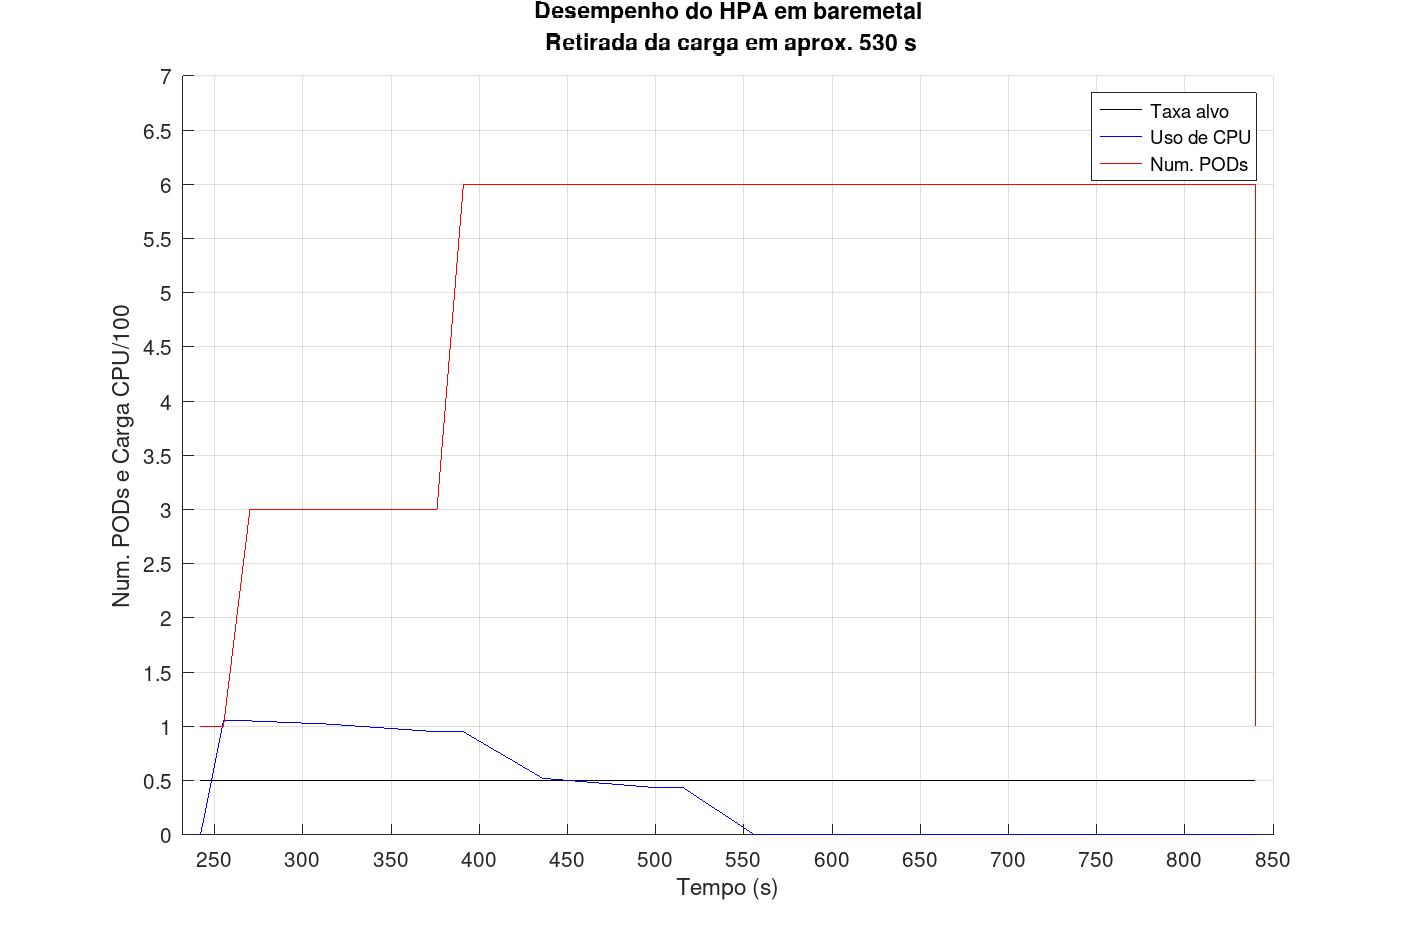
\includegraphics[width=.9\textwidth]{baremetal.png}
\caption{Resultados do teste de carga com kubernetes em ambiente \textit{baremetal}}
\label{fig:resultado-baremetal}
\end{figure}

\begin{figure}[htbp]
\centering
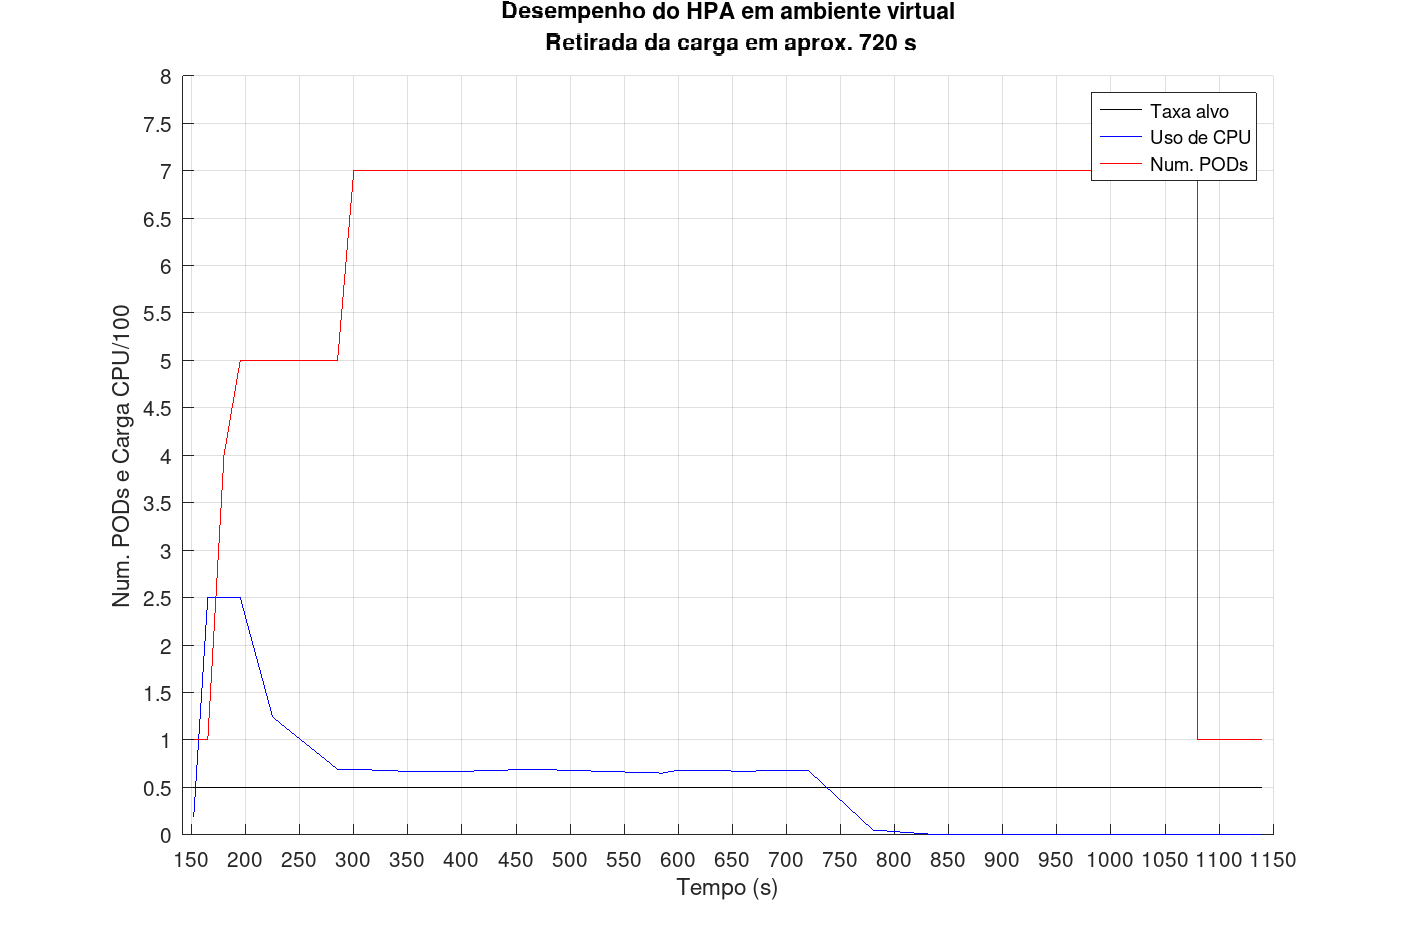
\includegraphics[width=.9\textwidth]{ambiente_virtual.png}
\caption{Resultado do teste de carga com kubernetes em ambiente virtualizado}
\label{fig:resultado-vm}
\end{figure}

\subsection{HPA na Amazon EKS}

O Amazon Elastic Kubernetes Service é o serviço de nuvem da Amazon AWS para implementação de clusters Kubernetes escaláveis, abstraindo a necessidade de criação e gerenciamento da infraestrutura de rede e servidor. A documentação de criação e gerenciamento dos clusters no Amazon EKS está disponível no \textit{site} da AWS \cite{amazon_getting_nodate}.

A nuvem Amazon AWS permite a criação de clusters no EKS de diferentes maneiras. Pode-se criá-los usando a interface \textit{web} de gerenciamento da Amazon EKS (Figura~\ref{fig:interface-amazon-eks}, o utilitário \textit{eksctl}, disponibilizado pela Amazon AWS, ou ainda o utilitário de gerenciamento em nuvem \textit{aws cli}. Os testes realizados utilizaram a ferramenta \textit{aws cli} e a interface de gerenciamento em nuvem.

\begin{figure}[htbp]
\centering
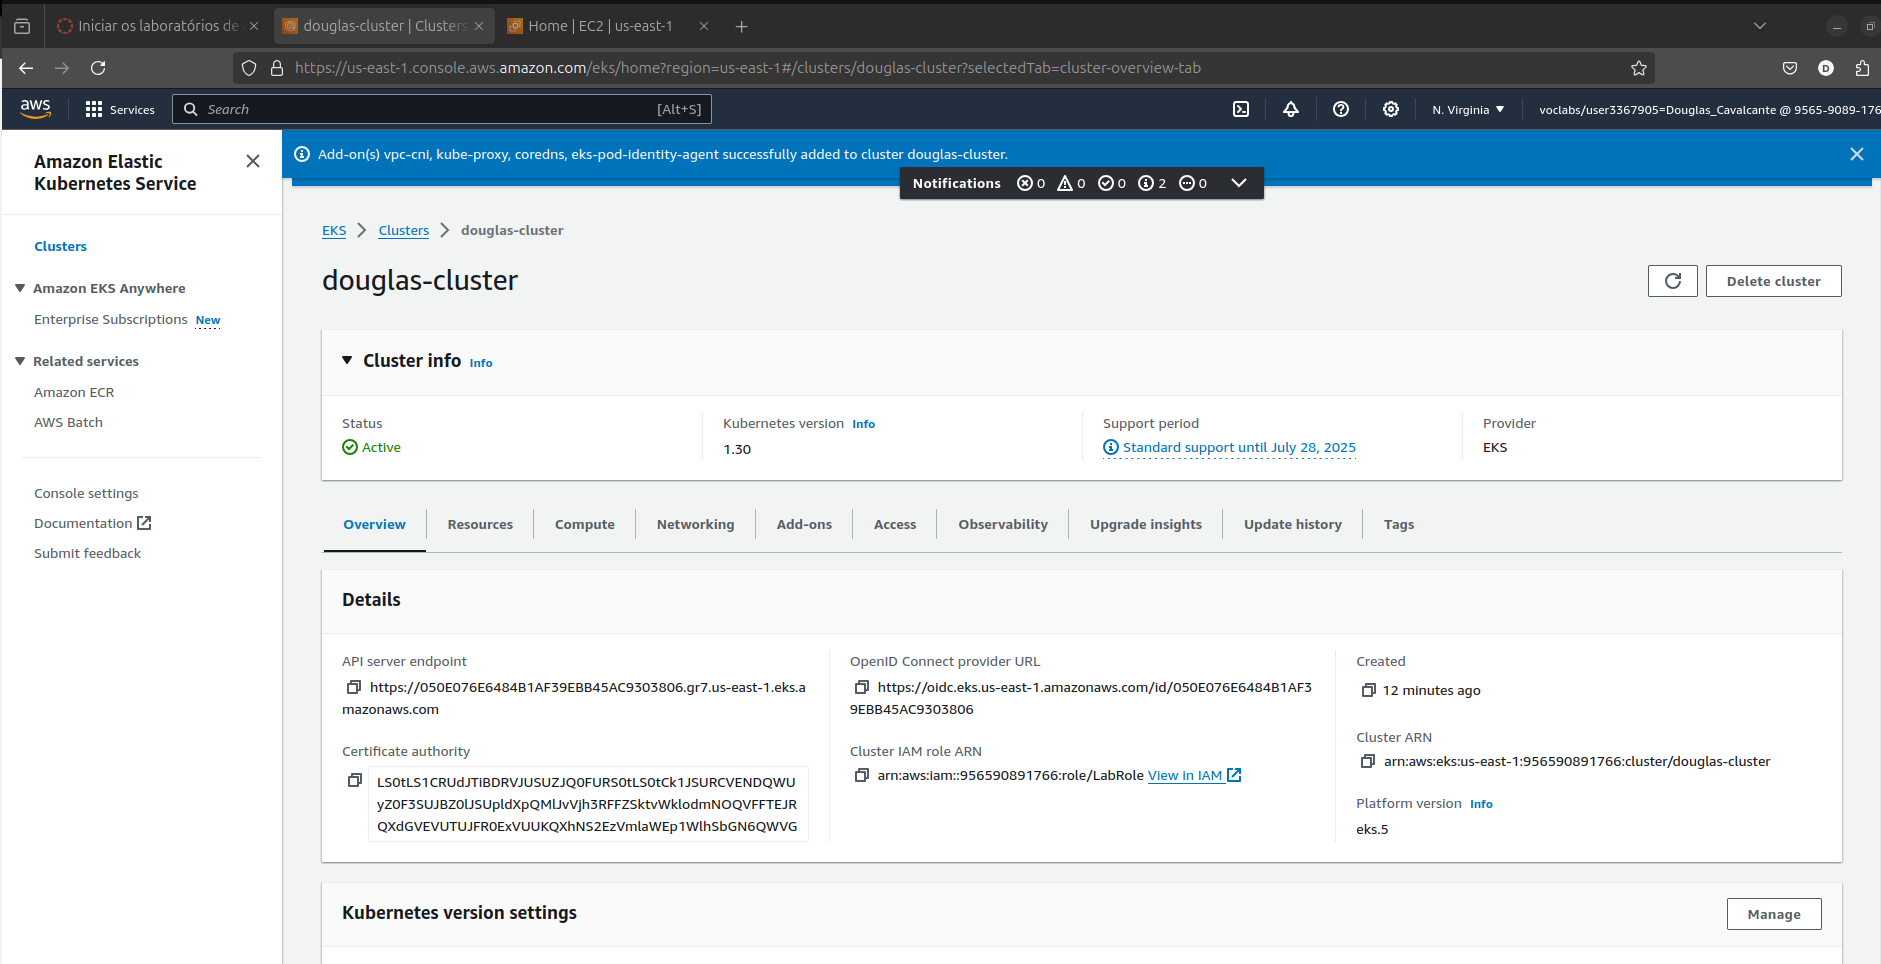
\includegraphics[width=.9\textwidth]{douglas-cluster.png}
\caption{Interface de gerenciamento e criação de clusters na Amazon EKS}
\label{fig:interface-amazon-eks}
\end{figure}

A conta utilizada para criação do cluster na Amazon EKS, bem como para execução dos testes, foi a disponibilizada pela Amazon para os alunos da disciplina PSI5120-2024. Essa conta possui limitações de uso e não permite a criação de usuários e perfis (\textit{roles}), sendo que para os testes foram utilizados os usuários disponibilizados aos autores e a \textit{role} IAM LabRole.

\subsubsection{Criação do Cluster na Amazon EKS}

A criação do cluster se inicia com a formação de uma nuvem privada virtual (VPC) com subredes privadas que atendem os requisitos da Amazon EKS. Para isso, executa-se o comando \verb|$ aws cloudformation create-stack| com argumentos de região (utilizada a \textit{us-east-1}), nome da VPC e \textit{template} (utilizado o padrão sugerido no tutorial \cite{amazon_getting_nodate}).

Uma vez criada a VPC, cria-se o cluster utilizando a interface \textit{web} de gerenciamento da nuvem Amazon AWS, conforme mostrado na Figura~\ref{fig:interface-amazon-eks}. Sugere-se, então, configurar o ambiente para operação a partir da máquina local, criando um contexto de configuração do \textit{kubectl} para operação remota do cluster. Faz-se isso utilizando o comando \verb|$ aws eks update-kubeconfig|, informando a região e o nome do cluster.

\subsubsection{Criação dos Nós do Cluster na Amazon EC2}

A Amazon EKS fornece duas opções para criação de nós para o cluster, uma utilizando máquinas virtuais criadas no serviço Amazon Elastic Compute Cloud (EC2), e outra utilizando o Amazon Fargate. O Amazon Fargate é um serviço de computação \textit{serverless} que permite o \textit{deploy} de aplicações Kubernetes sem necessidade de uso de instânicas do EC2. Para os testes realizados nesse artigo foram utilizadas instâncias do EC2. Os nós do cluster são criados a partir do seu próprio ambiente de configuração na interface de gerenciamento (aba \textit{Compute} do Amazon EKS). Para os testes em questão foram criadas duas instâncias do tipo \textit{t3.medium} com quantidades padrões de cpu e memória.

\subsubsection{Deploy da Aplicação e Configuração do HPA}

O \textit{deploy} da aplicação de testes \textit{php-apache} e a configuração do HPA seguiram exatamente os procedimentos relatados na Seção~\ref{subsec:hpa}, depois de criados os nós e configurado o \textit{kubectl}, conforme explicado na subseção anterior.

\subsubsection{Teste de Escalonamento Horizontal}

Da mesma forma que descrito na Seção~\ref{subsec:teste-hpa-local}, o teste de escalonamento horizontal consistiu na criação de um pod que efetuava requisições http em intervalos de 0,01~ms, sendo que esse pod foi criado no cluster na Amazon EKS conforme o procedimento do \textit{site} da Amazon AWS \cite{amazon_scale_nodate}. A Figura~\ref{fig:resultado-aws-eks} mostra o comportamento do HPA obtido o ambiente Amazon EKS de um dos autores\footnote{Consultar o repositório do projeto para visualização dos testes realizados por ambos os autores.}.

\begin{figure}[htbp]
\centering
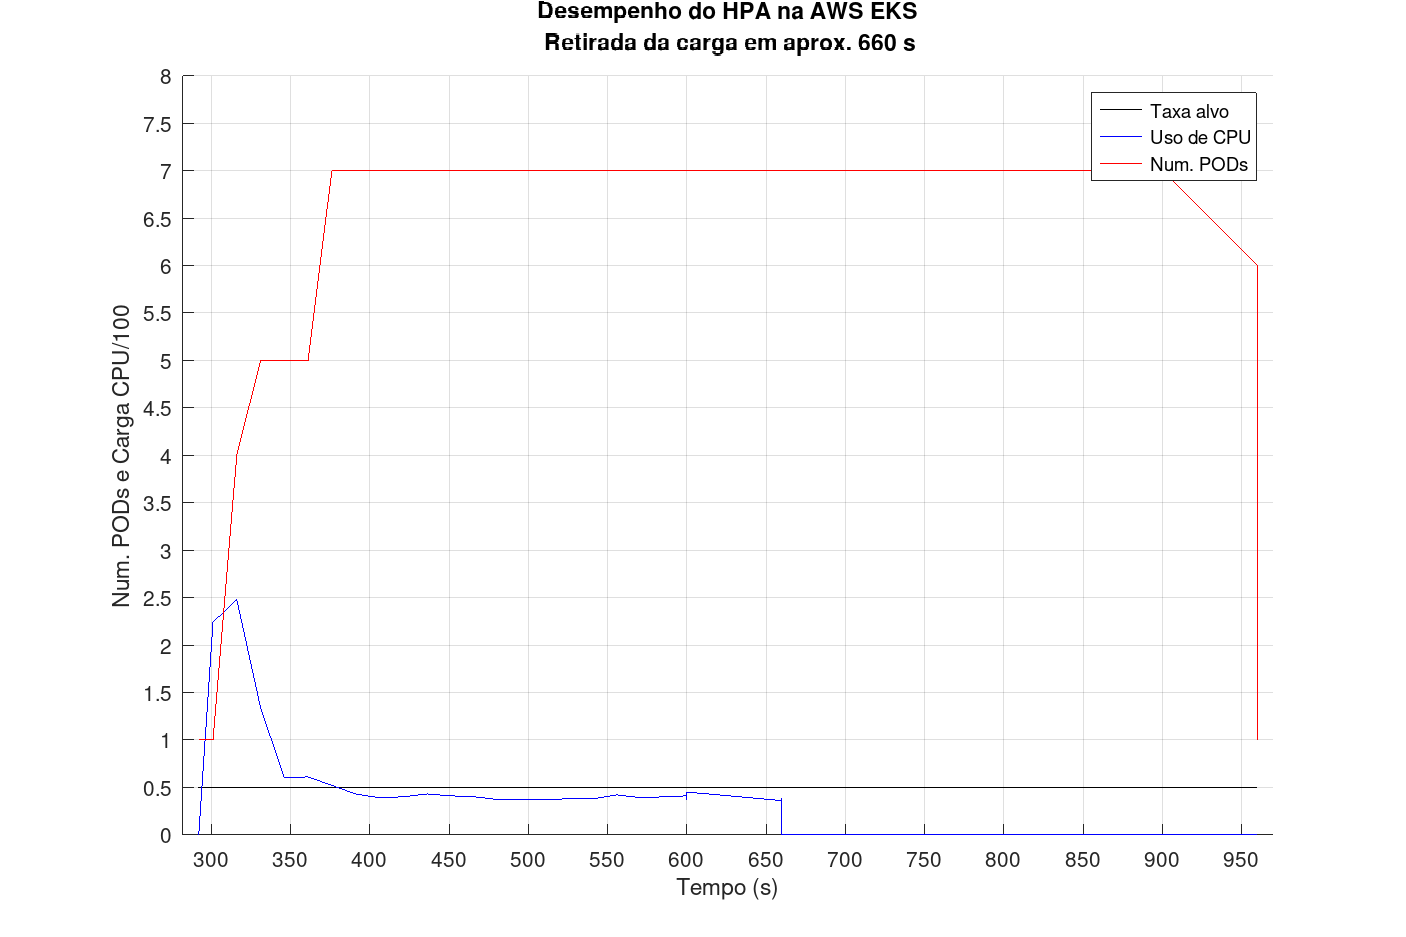
\includegraphics[width=.9\textwidth]{aws_eks.png}
\caption{Resultados do teste de carga com Kubernetes na Amazon EKS}
\label{fig:resultado-aws-eks}
\end{figure}

\section{Análise de Resultados} \label{sec:analise-resultados}

A Tabela~\ref{tab:respostas-hpa} mostra os resultados obtidos para os três ambientes implementados, contendo a média de carga percentual da CPU durante o período de maior número de réplicas e o tempos de criação e de remoção dos pods, dados esses também representados nas Figuras~\ref{fig:resultado-baremetal},~\ref{fig:resultado-vm}~e~\ref{fig:resultado-aws-eks}.

\begin{table}[htbp]
\centering
\caption{Respostas do HPA nas três condições testadas}
\label{tab:respostas-hpa}

    \begin{tabular}{|l|r|r|r|r|}
        \hline
        \textbf{Ambiente} & \textbf{Média \% CPU} &\textbf{Criação pod (s)} &\textbf{ Rem. pods} & \textbf{Máx réplicas}\\ \hline
        \textit{Baremetal} & 46,7 & 149 & 325 & 6  \\ \hline
        Ambiente virtual & 67,4 & 148 & 240 & 7 \\ \hline
        Amazon AWS/EKS & 40,7 & 84 & 300 & 7 \\ \hline
    \end{tabular}

\end{table}

Observa-se que, para as implementações em ambiente local, a média da carga de CPU em \textit{{baremetal}} é menor em relação ao ambiente virtualizado, que, por sua vez, tem um tempo remanescente de réplicas menor quando a carga no servidor \textit{web} é removida. A implementação em nuvem Amazon AWS com EKS manteve cargas menores em relação aos ambientes locais e apresentou tempo para criação das réplicas 43,2~\% menor que os obtidos nos ambientes locais, porém o tempo de remoção foi similar (cabe ressaltar que a documentação da Amazon EKS ressalta que a resposta à redução de carga pode levar até 5~minutos \cite{amazon_scale_nodate}). Ressalta-se, ainda, que o ambiente em \textit{baremetal} conseguiu estabilizar a carga de CPU perto da meta de 50~\% com uma réplica a menos.

Embora a plataforma Kubernetes tenha o mesmo processo de instalação para as implementações locais, que se utilizam de ambiente \textit{{baremetal}} e virtualizado, o comportamento de evolução da carga e das réplicas pode ser distinto. A implementação de um servidor \textit{web} em Kubernetes em uma infraestrutura \textit{{baremetal}} tende a oferecer desempenho superior, pois elimina a camada de virtualização e permite acesso direto aos recursos de hardware, podendo resultar em menor latência e maior \textit{throughput}. Esse comportamento se mostrou presente nos testes realizados, conforme pode ser visto na Tabela~\ref{tab:respostas-hpa}, onde o mesmo desempenho foi obtido com um pod a menos. No entanto, abordagem \textit{baremetal} pode ser mais complexa na configuração inicial e no gerenciamento contínuo do hardware. Por outro lado, ao utilizar um ambiente virtualizado tende-se haver uma perda de desempenho devido à virtualização, mas ganha-se em flexibilidade e isolamento. A virtualização facilita a criação, destruição e migração de máquinas virtuais, o que pode ser vantajoso em ambientes dinâmicos.

%%% Penso que o próximo parágrafo está redudante... sugiro retirarmos.

%Enquanto o \textit{{baremetal}} permite uma escalabilidade física direta e otimiza o uso de recursos a longo prazo, a virtualização com KVM oferece uma escalabilidade mais flexível, permitindo a adição de recursos virtuais sem a necessidade imediata de novo hardware. No entanto, essa flexibilidade vem acompanhada de custos adicionais e potencialmente maior complexidade na configuração do ambiente. A escolha entre as duas abordagens depende dos requisitos específicos do projeto, como a necessidade de desempenho, controle sobre o hardware, flexibilidade e isolamento.

Já na implementação do mesmo servidor \textit{web} em Kubernetes utilizando Amazon AWS/EKS sobre instâncias EC2 combina a flexibilidade e o poder da infraestrutura em nuvem com o gerenciamento simplificado do Kubernetes, o que permite mitigar possíveis perdas de desempenho. O Amazon AWS/EKS gerencia a configuração e o controle da camada de Kubernetes, permitindo que as equipes se concentrem no desenvolvimento e na operação das aplicações sem se preocupar com a complexidade da gestão do cluster. As instâncias EC2 fornecem a capacidade de escalar automaticamente com base na demanda, que simplifica a implementação no geral.

\section{Conclusão}\label{sec:conclusao}

Considerando as implementações realizadas, a escolha da infraestrutura para um servidor \textit{web} em Kubernetes envolve uma análise cuidadosa das necessidades de desempenho, flexibilidade, escalabilidade e custos. A implementação em \textit{{baremetal}} proporciona desempenho máximo com acesso direto ao hardware, sendo ideal para cargas de trabalho que exigem latência mínima. Contudo, essa abordagem pode ser mais complexa de gerenciar e menos flexível em termos de escalabilidade rápida. Por outro lado, a virtualização oferece maior flexibilidade e isolamento, permitindo um gerenciamento mais ágil das máquinas virtuais, embora com uma penalidade de desempenho devido ao \textit{overhead} da virtualização.

Por outro lado, a implementação em nuvem, utilizando o Amazon AWS/EKS em instâncias EC2 destaca-se por permitir que os recursos se ajustem dinamicamente à demanda de forma tecnicamente ilimitada, o que é essencial para aplicações com cargas de trabalho variáveis. Percebeu-se pelos resultados dos testes que as variações de desempenho necessariamente levam a análises de custo-benefício para a melhor escolha.

A decisão entre implementação local ou na nuvem deve considerar o equilíbrio entre a necessidade de controle e otimização de recursos oferecida pelas soluções locais e a flexibilidade e escalabilidade proporcionada pela nuvem.

\bibliographystyle{sbc}
\bibliography{sbc-template}

\end{document}
